%\documentclass[a4paper, 11pt]{article}

%\include{jtex}
%\usepackage{tikz,ifthen}
%\usetikzlibrary{arrows,positioning,shapes,topaths,calc,fit,backgrounds,matrix,shadows}

%\begin{document}

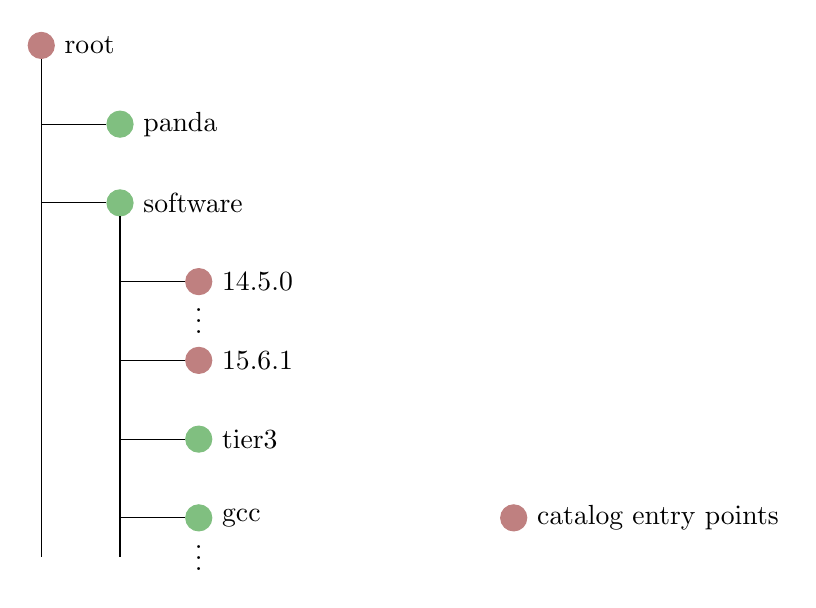
\begin{tikzpicture}
	[
		dirent/.style={
			circle,
			draw=green!50!black!50,
			fill=green!50!black!50
		}
	]
	\node[dirent,label=right:root,red!50!black!50,fill=red!50!black!50] (root) at (0,0) {};
	\node[dirent,label=right:panda] (panda) at (1, -1) {};
	\node[dirent,label=right:software] (software) at (1, -2) {};
	\node[dirent,label=right:14.5.0,red!50!black!50,fill=red!50!black!50] (1450) at (2, -3) {};
	\node[] (dots1) at (2, -3.4) {$\vdots$};
	\node[dirent,label=right:15.6.1,red!50!black!50,fill=red!50!black!50] (1561) at (2, -4) {};
	\node[dirent,label=right:tier3] (tier3) at (2, -5) {};
	\node[dirent,label=right:gcc] (gcc) at (2, -6) {};
	\node[] (dots2) at (2, -6.4) {$\vdots$};
	\node[dirent,label=right:catalog entry points,red!50!black!50,fill=red!50!black!50] (key) at (6,-6) {};
	
	%\node[dirent] (d2) at (0.4, 0.8) {};
	%\node[dirent,red!50!black!50,fill=red!50!black!50] (d21) at (0.8, 0.4) {};
	%\node[dirent] (d22) at (0.8, 0) {};
	%\node[scale=0.175] (file) at (2, 0.8) {\pdfimage{file.pdf}};
	
	\draw (root) -- (0,-1) -- (panda);
	\draw (0,-1) -- (0,-2) -- (software);
	\draw (0,-2) -- (0,-6.5);
	\draw (software) -- (1,-3) -- (1450);
	\draw (1,-3) -- (1,-4) -- (1561);
	\draw (1,-4) -- (1,-5) -- (tier3);
	\draw (1,-5) -- (1,-6) -- (gcc);
	\draw (1,-6) -- (1,-6.5);
\end{tikzpicture}
%\end{document}